
\documentclass[lineno]{jfm}

\usepackage{graphicx}
%\usepackage{epstopdf,epsfig}
\usepackage{newtxtext}
\usepackage{newtxmath}
\usepackage{natbib}
\usepackage{hyperref}
\hypersetup{
    colorlinks = true,
    urlcolor   = blue,
    citecolor  = black,
}
\newtheorem{lemma}{Lemma}
\newtheorem{corollary}{Corollary}
\newcommand{\RomanNumeralCaps}[1]
\linenumbers

% {\MakeUppercase{\romannumeral #1}}

\title{JFM {\LaTeX} submission template}

\author{Alan N. Jones\aff{1}
  \corresp{\email{JFMEditorial@cambridge.org}},
  H.-C. Smith\aff{1}
 \and J.Q. Long\aff{2}}

\affiliation{\aff{1}STM Journals, Cambridge University Press, The Printing House, Shaftesbury Road, Cambridge CB2 8BS, UK
\aff{2}DAMTP, Centre for Mathematical Sciences, Wilberforce Road, Cambridge CB3 0WA, UK}

\begin{document}
\maketitle

\begin{abstract}
This is the abstract.
\end{abstract}

\begin{keywords}
Authors should not enter keywords on the manuscript, as these must be chosen by the author during the online submission process and will then be added during the typesetting process (see \href{https://www.cambridge.org/core/journals/journal-of-fluid-mechanics/information/list-of-keywords}{Keyword PDF} for the full list).  Other classifications will be added at the same time.
\end{keywords}

{\bf MSC Codes }  {\it(Optional)} Please enter your MSC Codes here

\section{Introduction}
\label{sec:introduction}

First, we seek to generate a new Reynolds-averaged Navier--Stokes (RANS)
turbulence model that accurately predicts a turbulent DNS flow field.
We do this by creating new PDE terms based on the mean velocity and pressure
fields,
then use a simple regression technique to solve for the coefficients of
these terms.

Then, we simulate the flow field with this new model, showing how it is
much more accurate than a laminar model, i.e., one with no turbulence
parameterization.

\subsection {Second-order Heading}
 This is an example of dummy text. This is an example of dummy text. This is an example of dummy text. This is an example of dummy text. This is an example of dummy text. This is an example of dummy text. This is an example of dummy text. This is an example of dummy text. This is an example of dummy text. This is an example of dummy text. This is an example of dummy text. This is an example of dummy text.  This is an example of dummy text. This is an example of dummy text. This is an example of dummy text. This is an example of dummy text. This is an example of dummy text. This is an example of dummy text. This is an example of dummy text. This is an example of dummy text. This is an example of dummy text. This is an example of dummy text. This is an example of dummy text. This is an example of dummy text. This is an example of dummy text. This is an example of dummy text. This is an example of dummy text. This is an example of dummy text. This is an example of dummy text. This is an example of dummy text. This is an example of dummy text. This is an example of dummy text.

 \subsubsection {Third-order Heading}
 This is an example of dummy text. This is an example of dummy text. This is an example of dummy text. This is an example of dummy text. This is an example of dummy text. This is an example of dummy text. This is an example of dummy text. This is an example of dummy text. This is an example of dummy text. This is an example of dummy text. This is an example of dummy text. This is an example of dummy text. This is an example of dummy text. This is an example of dummy text. This is an example of dummy text. This is an example of dummy text. This is an example of dummy text. This is an example of dummy text. This is an example of dummy text. This is an example of dummy text. This is an example of dummy text. This is an example of dummy text. This is an example of dummy text. This is an example of dummy text. This is an example of dummy text. This is an example of dummy text. This is an example of dummy text. This is an example of dummy text. This is an example of dummy text. This is an example of dummy text. This is an example of dummy text.
\section{Figures and Tables}\label{sec:Figures_Tables}

\begin{figure}
  \centerline{\includegraphics{../figures/bl-profile-dns}}% Images in 100% size
  \caption{Trapped-mode wavenumbers, $kd$, plotted against $a/d$ for
    three ellipses:\protect\\
    ---$\!$---,
    $b/a=1$; $\cdots$\,$\cdots$, $b/a=1.5$.}
\label{fig:ka}
\end{figure}

\subsection{Figures}
 Each figure should be accompanied by a single caption, to appear beneath, and must be cited in the text. Figures should appear in the order in which they are first mentioned in the text. For example see figures \ref{fig:ka} and \ref{fig:kd}.

 This is an example of dummy text. This is an example of dummy text. This is an example of dummy text. This is an example of dummy text. This is an example of dummy text. This is an example of dummy text. This is an example of dummy text. This is an example of dummy text. This is an example of dummy text. This is an example of dummy text. This is an example of dummy text. This is an example of dummy text. This is an example of dummy text. This is an example of dummy text. This is an example of dummy text. This is an example of dummy text. This is an example of dummy text. This is an example of dummy text. This is an example of dummy text. This is an example of dummy text. This is an example of dummy text. This is an example of dummy text. This is an example of dummy text. This is an example of dummy text. This is an example of dummy text. This is an example of dummy text. This is an example of dummy text. This is an example of dummy text. This is an example of dummy text. This is an example of dummy text. This is an example of dummy text. This is an example of dummy text. This is an example of dummy text. This is an example of dummy text. This is an example of dummy text. This is an example of dummy text. This is an example of dummy text. This is an example of dummy text. This is an example of dummy text. This is an example of dummy text. This is an example of dummy text. This is an example of dummy text. This is an example of dummy text. This is an example of dummy text. This is an example of dummy text. This is an example of dummy text. This is an example of dummy text. This is an example of dummy text. This is an example of dummy text. This is an example of dummy text. This is an example of dummy text. This is an example of dummy text. This is an example of dummy text. This is an example of dummy text. This is an example of dummy text. This is an example of dummy text. This is an example of dummy text. This is an example of dummy text. This is an example of dummy text. This is an example of dummy text.

\begin{figure}
  \centerline{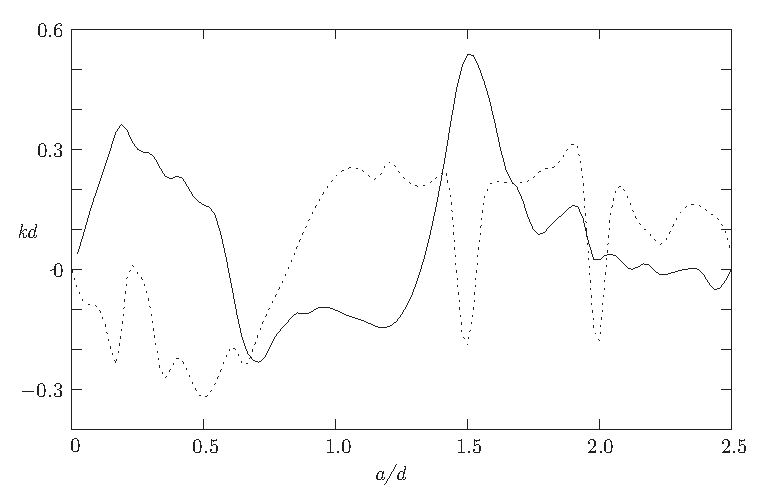
\includegraphics{Fig2}}
  \caption{The features of the four possible modes corresponding to
  (\textit{a}) periodic\protect\\ and (\textit{b}) half-periodic solutions.}
\label{fig:kd}
\end{figure}

\subsection{Tables}
 Tables, however small, must be numbered sequentially in the order in which they are mentioned in the text. Words \textit {table 1, table 2} should be lower case throughout.
 See table \ref{tab:kd} for an example.

 This is an example of dummy text. This is an example of dummy text. This is an example of dummy text. This is an example of dummy text. This is an example of dummy text. This is an example of dummy text. This is an example of dummy text. This is an example of dummy text. This is an example of dummy text. This is an example of dummy text. This is an example of dummy text. This is an example of dummy text. This is an example of dummy text. This is an example of dummy text. This is an example of dummy text. This is an example of dummy text. This is an example of dummy text. This is an example of dummy text. This is an example of dummy text. This is an example of dummy text. This is an example of dummy text. This is an example of dummy text. This is an example of dummy text. This is an example of dummy text. This is an example of dummy text. This is an example of dummy text. This is an example of dummy text. This is an example of dummy text. This is an example of dummy text. This is an example of dummy text. This is an example of dummy text. This is an example of dummy text. This is an example of dummy text. This is an example of dummy text. This is an example of dummy text. This is an example of dummy text. This is an example of dummy text. This is an example of dummy text. This is an example of dummy text. This is an example of dummy text. This is an example of dummy text. This is an example of dummy text. This is an example of dummy text. This is an example of dummy text. This is an example of dummy text. This is an example of dummy text. This is an example of dummy text. This is an example of dummy text. This is an example of dummy text. This is an example of dummy text. This is an example of dummy text. This is an example of dummy text. This is an example of dummy text. This is an example of dummy text. This is an example of dummy text. This is an example of dummy text. This is an example of dummy text. This is an example of dummy text. This is an example of dummy text. This is an example of dummy text.

\begin{table}
  \begin{center}
\def~{\hphantom{0}}
  \begin{tabular}{lccc}
      $a/d$  & $M=4$   &   $M=8$ & Callan \etal \\[3pt]
       0.1   & 1.56905 & ~~1.56~ & 1.56904\\
       0.3   & 1.50484 & ~~1.504 & 1.50484\\
       0.55  & 1.39128 & ~~1.391 & 1.39131\\
       0.7   & 1.32281 & ~10.322 & 1.32288\\
       0.913 & 1.34479 & 100.351 & 1.35185\\
  \end{tabular}
  \caption{Values of $kd$ at which trapped modes occur when $\rho(\theta)=a$.}
  \label{tab:kd}
  \end{center}
\end{table}

\section{Notation and style}\label{notstyle}
 Generally any queries concerning notation and journal style can be answered by viewing recent pages in the Journal. However, the following guide provides the key points to note. It is expected that Journal style and mathematical notation will be followed, and authors should take care to define all variables or entities upon first use. Also note that footnotes are not normally accepted.  Abbreviations must be defined at first use, glossaries or lists/tables of abbreviations are not permitted.

\subsection{Mathematical notation}
\subsubsection{Setting variables, functions, vectors, matrices etc}
\begin{itemize} \label{sec:MathNot}
\item {\bf Italic font} should be used for denoting variables, with multiple-letter symbols avoided except in the case of dimensionless numbers such as $\Rey$, $\Pran$ and $\Pen$ (Reynolds, Prandtl, and P\'eclet numbers respectively, which are defined as \verb}\Rey}, \verb}\Pran} and \verb}\Pen} in the template).\\
\item {\bf Upright Roman font} (or upright Greek where appropriate) should be used for:\\
\begin {enumerate}
\item (vI) label, e.g.  T. t (transpose)\\
\item Fixed operators: sin, log, d, $\Delta$, exp etc.\\
\item Constants: i ($\sqrt{-1}$), $\upi$ (defined as \verb}\upi}),e  etc.\\
\item Special Functions: $\Ai$, $\Bi$ (Airy functions, defined as \verb}\Ai} and \verb}\Bi}), $\Real$ (real part, defined as \verb}\Real}), $\Imag$ (imaginary part, defined as \verb}\Imag}), etc.\\[-4pt]
\item Physical units: cm, s, etc.\\[-4pt]
\item Abbreviations: c.c. (complex conjugate), h.o.t. (higher-order terms), DNS, etc.\\[-4pt]
\end {enumerate}
\item {\bf Bold italic font} (or bold sloping Greek) should be used for vectors (with the centred dot for a scalar product also in bold): $\boldsymbol{i \cdot j}$\\[-4pt]
\item {\bf Bold sloping sans serif font}, defined by the \verb}\mathsfbi} macro, should be used for tensors and matrices: $\mathsfbi{D}$ \\[-4pt]
\item {\bf Calligraphic font} (for example $\mathcal{G}$, $\mathcal{R}$) can be used as an alternative to italic when the same letter denotes a different quantity use \verb}\mathcal} in \LaTeX)
\end{itemize}

\subsubsection{Other symbols}  Large numbers  that are not scientific powers should not include commas, but should use a non-breaking space, and use the form 1600 or 16 000 or 160 000.
Use \textit{O} to denote `of the order of', not the \LaTeX\ $\mathcal{O}$.

The product symbol ($\times$) should only be used to denote multiplication where an equation is broken over more than one line, to denote a cross product, or between numbers . The $\boldsymbol {\cdot}$ symbol should not be used, except to denote a scalar product of vectors specifically.

\subsubsection{Example Equations}
 This section contains sample equations in the JFM style. Please refer to the {\LaTeX} source file for examples of how to display such equations in your manuscript.

\begin{equation}
  (\nabla^2+k^2)G_s=(\nabla^2+k^2)G_a=0
  \label{Helm}
\end{equation}

\begin{equation}
  \bnabla\bcdot\boldsymbol{v} = 0,\quad \nabla^{2}P=
    \bnabla\bcdot(\boldsymbol{v}\times \boldsymbol{w}).
\end{equation}

\begin{equation}
  G_s,G_a\sim 1 / (2\upi)\ln r
  \quad \mbox{as\ }\quad r\equiv|P-Q|\rightarrow 0,
  \label{singular}
\end{equation}

\begin{equation}
\left. \begin{array}{ll}
\displaystyle\frac{\p G_s}{\p y}=0
  \quad \mbox{on\ }\quad y=0,\\[8pt]
\displaystyle  G_a=0
  \quad \mbox{on\ }\quad y=0,
 \end{array}\right\}
  \label{symbc}
\end{equation}

\begin{equation}
  -\frac{1}{2\upi} \int_0^{\infty} \gamma^{-1}[\mathrm exp(-k\gamma|y-\eta|)
   + \mathrm exp(-k\gamma(2d-y-\eta))] \cos k(x-\xi)t\:\mathrm{d} t,
   \qquad 0<y,\quad \eta<d,
\end{equation}

\begin{equation}
  \gamma(t) = \left\{
    \begin{array}{ll}
      -\mathrm{i}(1-t^2)^{1/2}, & t\le 1 \\[2pt]
      (t^2-1)^{1/2},         & t>1.
    \end{array} \right.
\end{equation}

\[
  -\frac{1}{2\upi}
   \pvi B(t)\frac{\cosh k\gamma(d-y)}{\gamma\sinh k\gamma d}
   \cos k(x-\xi)t\:\mathrm{d} t
\]

\begin{equation}
  G = -\frac{1}{4}\mathrm{i} (H_0(kr)+H_0(kr_1))
    - \frac{1}{\upi} \pvi\frac{\mathrm{e}^{-\kgd}}%
    {\gamma\sinh\kgd} \cosh k\gamma(d-y) \cosh k\gamma(d-\eta)
\end{equation}

Note that when equations are included in definitions, it may be suitable to render them in line, rather than in the equation environment: $\boldsymbol{n}_q=(-y^{\prime}(\theta),
x^{\prime}(\theta))/w(\theta)$.
Now $G_a=\squart Y_0(kr)+\Gat$ where
$r=\{[x(\theta)-x(\psi)]^2 + [y(\theta)-y(\psi)]^2\}^{1/2}$ and $\Gat$ is
regular as $kr\ttz$. However, any fractions displayed like this, other than $\thalf$ or $\squart$, must be written on the line, and not stacked (ie 1/3).

\begin{eqnarray}
  \ndq\left(\frac{1}{4} Y_0(kr)\right) & \sim &
    \frac{1}{4\upi w^3(\theta)}
    [x^{\prime\prime}(\theta)y^{\prime}(\theta)-
    y^{\prime\prime}(\theta)x^{\prime}(\theta)] \nonumber\\
  & = & \frac{1}{4\upi w^3(\theta)}
    [\rho^{\prime}(\theta)\rho^{\prime\prime}(\theta)
    - \rho^2(\theta)-2\rho^{\prime 2}(\theta)]
    \quad \mbox{as\ }\quad kr\ttz . \label{inteqpt}
\end{eqnarray}

\begin{equation}
  \frac{1}{2}\phi_i = \frac{\upi}{M} \sumjm\phi_j K_{ij}^a w_j,
  \qquad i=1,\,\ldots,\,M,
\end{equation}
where
\begin{equation}
  K_{ij}^a = \left\{
    \begin{array}{ll}
      \p G_a(\theta_i,\theta_j)/\p n_q, & i\neq j \\[2pt]
      \p\Gat(\theta_i,\theta_i)/\p n_q
      + [\rho_i^{\prime}\rho_i^{\prime\prime}-\rho_i^2-2\rho_i^{\prime 2}]
      / 4\upi w_i^3, & i=j.
  \end{array} \right.
\end{equation}


\refstepcounter{equation}
$$
  \rho_l = \lim_{\zeta \rightarrow Z^-_l(x)} \rho(x,\zeta), \quad
  \rho_{u} = \lim_{\zeta \rightarrow Z^{+}_u(x)} \rho(x,\zeta)
  \eqno{(\theequation{\mathit{a},\mathit{b}})}\label{eq35}
$$

\begin{equation}
  (\rho(x,\zeta),\phi_{\zeta\zeta}(x,\zeta))=(\rho_0,N_0)
  \quad \mbox{for}\quad Z_l(x) < \zeta < Z_u(x).
\end{equation}


\begin{subeqnarray}
  \tau_{ij} & = &
    (\overline{\overline{u}_i \overline{u}_j}
    - \overline{u}_i\overline{u}_j)
    + (\overline{\overline{u}_iu^{SGS}_j
    + u^{SGS}_i\overline{u}_j})
    + \overline{u^{SGS}_iu^{SGS}_j},\\[3pt]
  \tau^\theta_j & = &
    (\overline{\overline{u}_j\overline{\theta}}
    - \overline{u}_j \overline{\theta})
    + (\overline{\overline{u}_j\theta^{SGS}
    + u^{SGS}_j \overline{\theta}})
    + \overline{u^{SGS}_j\theta^{SGS}}.
\end{subeqnarray}

\begin{equation}
\setlength{\arraycolsep}{0pt}
\renewcommand{\arraystretch}{1.3}
\slsQ_C = \left[
\begin{array}{ccccc}
  -\omega^{-2}V'_w  &  -(\alpha^t\omega)^{-1}  &  0  &  0  &  0  \\
  \displaystyle
  \frac{\beta}{\alpha\omega^2}V'_w  &  0  &  0  &  0  &  \mathrm{i}\omega^{-1} \\
  \mathrm{i}\omega^{-1}  &  0  &  0  &  0  &  0  \\
  \displaystyle
  \mathrm{i} R^{-1}_{\delta}(\alpha^t+\omega^{-1}V''_w)  &  0
    & -(\mathrm{i}\alpha^tR_\delta)^{-1}  &  0  &  0  \\
  \displaystyle
  \frac{\mathrm{i}\beta}{\alpha\omega}R^{-1}_\delta V''_w  &  0  &  0
    &  0  & 0 \\
  (\mathrm{i}\alpha^t)^{-1}V'_w  &  (3R^{-1}_{\delta}+c^t(\mathrm{i}\alpha^t)^{-1})
    &  0  &  -(\alpha^t)^{-2}R^{-1}_{\delta}  &  0  \\
\end{array}  \right] .
\label{defQc}
\end{equation}

\begin{equation}
\etb^t = \skew2\hat{\etb}^t \exp [\mathrm{i} (\alpha^tx^t_1-\omega t)],
\end{equation}
where $\skew2\hat{\etb}^t=\boldsymbol{b}\exp (\mathrm{i}\gamma x^t_3)$.
\begin{equation}
\mbox{Det}[\rho\omega^2\delta_{ps}-C^t_{pqrs}k^t_qk^t_r]=0,
\end{equation}

\begin{equation}
 \langle k^t_1,k^t_2,k^t_3\rangle = \langle
\alpha^t,0,\gamma\rangle
\end{equation}

\begin{equation}
\boldsymbol{f}(\theta,\psi) = (g(\psi)\cos \theta,g(\psi) \sin \theta,f(\psi)).
\label{eq41}
\end{equation}

\begin{eqnarray}
f(\psi_1) = \frac{3b}{\upi[2(a+b \cos \psi_1)]^{{3}/{2}}}
  \int^{2\upi}_0 \frac{(\sin \psi_1 - \sin \psi)(a+b \cos \psi)^{1/2}}%
  {[1 - \cos (\psi_1 - \psi)](2+\alpha)^{1/2}}\mathrm{d}x,
\label{eq42}
\end{eqnarray}
\begin{eqnarray}
g(\psi_1) & = & \frac{3}{\upi[2(a+b \cos \psi_1)]^{{3}/{2}}}
  \int^{2\upi}_0 \left(\frac{a+b \cos \psi}{2+\alpha}\right)^{1/2}
  \left\{ \astrut f(\psi)[(\cos \psi_1 - b \beta_1)S + \beta_1P]
  \right. \nonumber\\
&& \mbox{}\times \frac{\sin \psi_1 - \sin \psi}{1-\cos(\psi_1 - \psi)}
  + g(\psi) \left[\left(2+\alpha - \frac{(\sin \psi_1 - \sin \psi)^2}
  {1- \cos (\psi - \psi_1)} - b^2 \gamma \right) S \right.\nonumber\\
&& \left.\left.\mbox{} + \left( b^2 \cos \psi_1\gamma -
  \frac{a}{b}\alpha \right) F(\frac{1}{2}\upi, \delta) - (2+\alpha)
  \cos\psi_1 E(\frac{1}{2}\upi, \delta)\right] \astrut\right\} \mathrm{d} \psi,
\label{eq43}
\end{eqnarray}
\begin{equation}
\alpha = \alpha(\psi,\psi_1) = \frac{b^2[1-\cos(\psi-\psi_1)]}%
  {(a+b\cos\psi) (a+b\cos\psi_1)},
  \quad
  \beta - \beta(\psi,\psi_1) = \frac{1-\cos(\psi-\psi_1)}{a+b\cos\psi}.
\end{equation}


\begin{equation}
\left. \begin{array}{l}
\displaystyle
H(0) = \frac{\epsilon \overline{C}_v}{\tilde{v}^{{1}/{2}}_T
(1- \beta)},\quad H'(0) = -1+\epsilon^{{2}/{3}} \overline{C}_u
+ \epsilon \skew5\hat{C}_u'; \\[16pt]
\displaystyle
H''(0) = \frac{\epsilon u^2_{\ast}}{\tilde{v}^{{1}/{2}}
_T u^2_P},\quad H' (\infty) = 0.
\end{array} \right\}
\end{equation}

\begin{lemma}
Let $f(z)$ be a trial \citet[][pp.~231--232]{Batchelor59} function defined on $[0,1]$.  Let $\varLambda_1$ denote
the ground-state eigenvalue for $-\mathrm{d}^2g/\mathrm{d} z^2=\varLambda g$,
where $g$ must satisfy $\pm\mathrm{d} g/\mathrm{d} z+\alpha g=0$ at $z=0,1$
for some non-negative constant~$\alpha$.  Then for any $f$ that is not
identically zero we have
\begin{equation}
\frac{\displaystyle
  \alpha(f^2(0)+f^2(1)) + \int_0^1 \left(
  \frac{\mathrm{d} f}{\mathrm{d} z} \right)^2 \mathrm{d} z}%
  {\displaystyle \int_0^1 f^2\mathrm{d} z}
\ge \varLambda_1 \ge
\left( \frac{-\alpha+(\alpha^2+8\upi^2\alpha)^{1/2}}{4\upi} \right)^2.
\end{equation}
\end{lemma}

\begin{corollary}
Any non-zero trial function $f$ which satisfies the boundary condition
$f(0)=f(1)=0$ always satisfies
\begin{equation}
  \int_0^1 \left( \frac{\mathrm{d} f}{\mathrm{d} z} \right)^2 \mathrm{d} z.
\end{equation}
\end{corollary}

\section{Citations and references}
All papers included in the References section must be cited in the article, and vice versa. Citations should be included as, for example ``It has been shown \citep{Rogallo81} that...'' (using the {\verb}\citep}} command, part of the natbib package) ``recent work by \citet{Dennis85}...'' (using {\verb}\citet}}).
The natbib package can be used to generate citation variations, as shown below.\\
\verb#\citet[pp. 2-4]{Hwang70}#:\\
\citet[pp. 2-4]{Hwang70} \\
\verb#\citep[p. 6]{Worster92}#:\\
\citep[p. 6]{Worster92}\\
\verb#\citep[see][]{Koch83, Lee71, Linton92}#:\\
\citep[see][]{Koch83, Lee71, Linton92}\\
\verb#\citep[see][p. 18]{Martin80}#:\\
\citep[see][p. 18]{Martin80}\\
\verb#\citep{Brownell04,Brownell07,Ursell50,Wijngaarden68,Miller91}#:\\
\citep{Brownell04,Brownell07,Ursell50,Wijngaarden68,Miller91}\\
\citep{Briukhanovetal1967}\\
\cite{Bouguet01}\\
\citep{JosephSaut1990}\\

The References section can either be built from individual \verb#\bibitem# commands, or can be built using BibTex. The BibTex files used to generate the references in this document can be found in the JFM {\LaTeX} template files folder provided on the website \href{https://www.cambridge.org/core/journals/journal-of-fluid-mechanics/information/author-instructions/preparing-your-materials}{here}.

Where there are up to ten authors, all authors' names should be given in the reference list. Where there are more than ten authors, only the first name should appear, followed by {\it {et al.}}


\backsection[Supplementary data]{\label{SupMat}Supplementary material and movies are available at \\https://doi.org/10.1017/jfm.2019...}

\backsection[Acknowledgements]{Acknowledgements may be included at the end of the paper, before the References section or any appendices. Several anonymous individuals are thanked for contributions to these instructions.}

\backsection[Funding]{Please provide details of the sources of financial support for all authors, including grant numbers. Where no specific funding has been provided for research, please provide the following statement: "This research received no specific grant from any funding agency, commercial or not-for-profit sectors." }

\backsection[Declaration of interests]{A Competing Interests statement is now mandatory in the manuscript PDF. Please note that if there are no conflicts of interest, the declaration in your PDF should read as follows: {\bf Declaration of Interests}. The authors report no conflict of interest.}

\backsection[Data availability statement]{The data that support the findings of this study are openly available in [repository name] at http://doi.org/[doi], reference number [reference number]. See JFM's \href{https://www.cambridge.org/core/journals/journal-of-fluid-mechanics/information/journal-policies/research-transparency}{research transparency policy} for more information}

\backsection[Author ORCIDs]{Authors may include the ORCID identifers as follows.  F. Smith, https://orcid.org/0000-0001-2345-6789; B. Jones, https://orcid.org/0000-0009-8765-4321}

\backsection[Author contributions]{Authors may include details of the contributions made by each author to the manuscript'}

\appendix

\section{}\label{appA}
 In order not to disrupt the narrative flow, purely technical material may be included in the appendices. This material should corroborate or add to the main result and be essential for the understanding of the paper. It should be a small proportion of the paper and must not be longer than the paper itself.

This is an example of dummy text. This is an example of dummy text. This is an example of dummy text. This is an example of dummy text. This is an example of dummy text. This is an example of dummy text. This is an example of dummy text. This is an example of dummy text. This is an example of dummy text. This is an example of dummy text. This is an example of dummy text. This is an example of dummy text. This is an example of dummy text. This is an example of dummy text. This is an example of dummy text. This is an example of dummy text. This is an example of dummy text. This is an example of dummy text. This is an example of dummy text. This is an example of dummy text. This is an example of dummy text. This is an example of dummy text. This is an example of dummy text. This is an example of dummy text. This is an example of dummy text. This is an example of dummy text. This is an example of dummy text. This is an example of dummy text. This is an example of dummy text. This is an example of dummy text. This is an example of dummy text. This is an example of dummy text. This is an example of dummy text. This is an example of dummy text. This is an example of dummy text. This is an example of dummy text. This is an example of dummy text. This is an example of dummy text. This is an example of dummy text. This is an example of dummy text. This is an example of dummy text. This is an example of dummy text. This is an example of dummy text. This is an example of dummy text. This is an example of dummy text. This is an example of dummy text. This is an example of dummy text. This is an example of dummy text. This is an example of dummy text. This is an example of dummy text. This is an example of dummy text. This is an example of dummy text. This is an example of dummy text. This is an example of dummy text. This is an example of dummy text. This is an example of dummy text. This is an example of dummy text. This is an example of dummy text. This is an example of dummy text. This is an example of dummy text. This is an example of dummy text. This is an example of dummy text. This is an example of dummy text. This is an example of dummy text. This is an example of dummy text. This is an example of dummy text. This is an example of dummy text. This is an example of dummy text. This is an example of dummy text. This is an example of dummy text. This is an example of dummy text. This is an example of dummy text. This is an example of dummy text. This is an example of dummy text. This is an example of dummy text. This is an example of dummy text. This is an example of dummy text. This is an example of dummy text. This is an example of dummy text. This is an example of dummy text. This is an example of dummy text. This is an example of dummy text. This is an example of dummy text. This is an example of dummy text. This is an example of dummy text. This is an example of dummy text. This is an example of dummy text. This is an example of dummy text. This is an example of dummy text. This is an example of dummy text. This is an example of dummy text. This is an example of dummy text. This is an example of dummy text. This is an example of dummy text. This is an example of dummy text. This is an example of dummy text. This is an example of dummy text. This is an example of dummy text. This is an example of dummy text. This is an example of dummy text.

This is an example of dummy text. This is an example of dummy text. This is an example of dummy text. This is an example of dummy text. This is an example of dummy text. This is an example of dummy text. This is an example of dummy text. This is an example of dummy text. This is an example of dummy text. This is an example of dummy text. This is an example of dummy text. This is an example of dummy text. This is an example of dummy text. This is an example of dummy text. This is an example of dummy text. This is an example of dummy text. This is an example of dummy text. This is an example of dummy text. This is an example of dummy text. This is an example of dummy text. This is an example of dummy text. This is an example of dummy text. This is an example of dummy text. This is an example of dummy text. This is an example of dummy text. This is an example of dummy text. This is an example of dummy text. This is an example of dummy text. This is an example of dummy text. This is an example of dummy text. This is an example of dummy text. This is an example of dummy text. This is an example of dummy text. This is an example of dummy text. This is an example of dummy text. This is an example of dummy text. This is an example of dummy text. This is an example of dummy text. This is an example of dummy text. This is an example of dummy text. This is an example of dummy text. This is an example of dummy text. This is an example of dummy text. This is an example of dummy text. This is an example of dummy text. This is an example of dummy text. This is an example of dummy text. This is an example of dummy text. This is an example of dummy text. This is an example of dummy text. This is an example of dummy text. This is an example of dummy text. This is an example of dummy text. This is an example of dummy text. This is an example of dummy text. This is an example of dummy text. This is an example of dummy text. This is an example of dummy text. This is an example of dummy text. This is an example of dummy text. This is an example of dummy text. This is an example of dummy text. This is an example of dummy text. This is an example of dummy text. This is an example of dummy text. This is an example of dummy text. This is an example of dummy text. This is an example of dummy text. This is an example of dummy text. This is an example of dummy text. This is an example of dummy text. This is an example of dummy text. This is an example of dummy text. This is an example of dummy text. This is an example of dummy text. This is an example of dummy text. This is an example of dummy text. This is an example of dummy text. This is an example of dummy text. This is an example of dummy text. This is an example of dummy text. This is an example of dummy text. This is an example of dummy text. This is an example of dummy text. This is an example of dummy text. This is an example of dummy text. This is an example of dummy text. This is an example of dummy text. This is an example of dummy text. This is an example of dummy text. This is an example of dummy text. This is an example of dummy text. This is an example of dummy text. This is an example of dummy text. This is an example of dummy text. This is an example of dummy text. This is an example of dummy text. This is an example of dummy text. This is an example of dummy text. This is an example of dummy text. This is an example of dummy text. This is an example of dummy text. This is an example of dummy text. This is an example of dummy text. This is an example of dummy text. This is an example of dummy text. This is an example of dummy text. This is an example of dummy text. This is an example of dummy text. This is an example of dummy text. This is an example of dummy text. This is an example of dummy text. This is an example of dummy text. This is an example of dummy text. This is an example of dummy text. This is an example of dummy text. This is an example of dummy text. This is an example of dummy text. This is an example of dummy text. This is an example of dummy text. This is an example of dummy text. This is an example of dummy text. This is an example of dummy text. This is an example of dummy text. This is an example of dummy text.

\bibliographystyle{jfm}
\bibliography{../references}
%Use of the above commands will create a bibliography using the .bib file. Shown below is a bibliography built from individual items.

\end{document}
